\documentclass[12pt]{article}
\usepackage[english]{babel}
\usepackage[utf8x]{inputenc}
\usepackage{fullpage}
\usepackage{graphicx}
\usepackage[version=3]{mhchem} 
\usepackage{siunitx} 
\usepackage{graphicx}
\usepackage{natbib} 
\usepackage{amsmath} 


\usepackage{listings}
\usepackage{color}

\title{Laboratory work nr. 3  \\Gready method and dynamic programming\\ } % Title

\author{\textsc{Bîrcu} \textsc{Maxim}} % Author name

\date{\today} % Date for the report

\definecolor{mygreen}{rgb}{0,0.6,0}
\definecolor{mygray}{rgb}{0.5,0.5,0.5}
\definecolor{mymauve}{rgb}{0.58,0,0.82}

\lstset{ %
  backgroundcolor=\color{white},   % choose the background color
  basicstyle=\footnotesize,        % size of fonts used for the code
  breaklines=true,                 % automatic line breaking only at whitespace
  captionpos=b,                    % sets the caption-position to bottom
  commentstyle=\color{mygreen},    % comment style
  escapeinside={\%*}{*)},          % if you want to add LaTeX within your code
  keywordstyle=\color{blue},       % keyword style
  stringstyle=\color{mymauve},     % string literal style
}

\begin{document}


\maketitle % Insert the title, author and date

\begin{center}
\begin{tabular}{l r}

Student: & Bîrcu Maxim \\ % Partner names
Instructor: & Cojanu Irina % Instructor/supervisor

\end{tabular}
\end{center}


\subsection*{Work purpose}
\subparagraph*{
\\1. Studying of the greedy technique  \\
2. Study of Dynamic programming\\
3. Implementation of Kruskal algorithm \\
4. Implementation of the Floyd algorithm\\
5. Comparison of the algorithms (time complexity diagram/table/empirical)}

\newpage
\section*{Results}

\subparagraph*{I've studied all greedy algorithms that I've implemented applying them to different graphs with different number of vertices, and computed the execution time for each of them to place all this data on a chart to see the main differences of those algorithms.
}

\section{Kruskal,Kruskal-Prim,Floyd and Djikstra algorithm implementation}

\subsection*{Source code in python}

\lstinputlisting[language=Python]{algorithms.py}

\section{Kruskal algorithm vs Kruskal-Prim}

\subsection*{
For better understanding of the results and to compare the algorithms easier I've computed the execution time for different graphs with different number of vertices and placed all this data on some graphs.
}


\begin{figure}[h!]
  \centering
    {%
      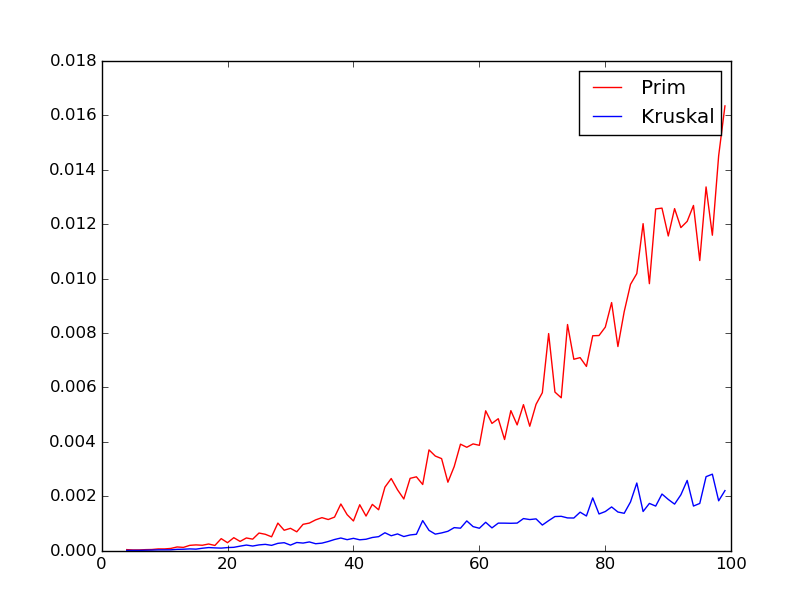
\includegraphics[width=0.5\textwidth]{1}}
\end{figure}

\begin{table}[h!]
  \begin{center}
    \begin{tabular}{|c|c|c|}
     \hline
      \text{Vertices} & \text{Kruskal} & \text{Kruskal-Prim}\\
       \hline
       4 & 1.3828277587890625e-05 & 4.100799560546875e-05  \\ 
       \hline
       5 & 1.0013580322265625e-05 & 1.4066696166992188e-05  \\ 
       \hline
       6 & 2.193450927734375e-05 & 4.601478576660156e-05  \\ 
       \hline
       7 & 2.193450927734375e-05 & 4.315376281738281e-05  \\ 
       \hline
       8 & 2.193450927734375e-05 & 6.103515625e-05  \\ 
       \hline
    \end{tabular}
  \end{center}
\end{table}

\subparagraph*{
From the graph above we can notice that Kruskal algorithm works quite fast in comparison with the Kruskal-Prime algorithm.
}
\newpage
\section{Floyd algorithm vs Dijkstra}

\subsection*{
For better understanding of the results and to compare the algorithms easier I've computed the execution time for different graphs with different number of vertices and placed all this data on some graphs.
}
\begin{figure}[h!]
  \centering
    {%
      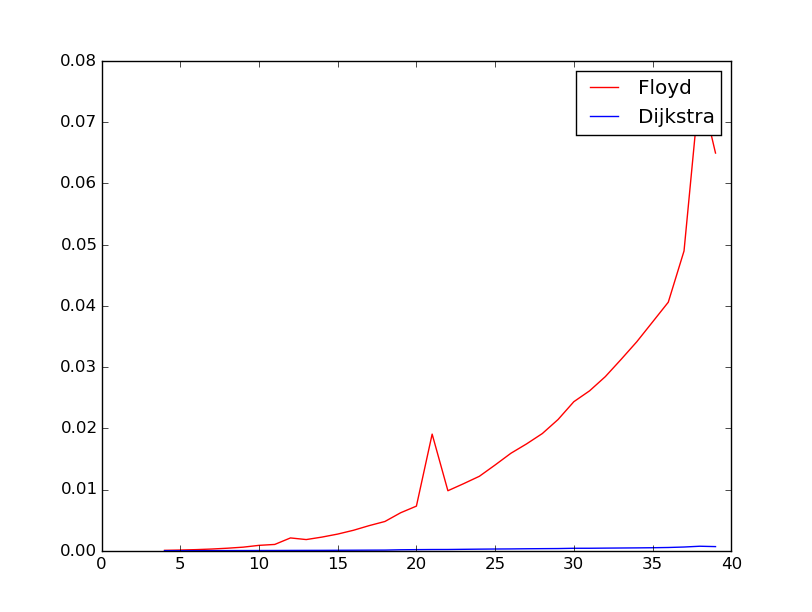
\includegraphics[width=0.5\textwidth]{2}}
\end{figure}

\begin{table}[h!]
  \begin{center}
    \begin{tabular}{|c|c|c|}
     \hline
      \text{Vertices} & \text{Floyd} & \text{Dijkstra}\\
       \hline
       4 & 1.2874603271484375e-05 & 3.886222839355469e-0  \\ 
       \hline
       5 & 2.09808349609375e-05 &  2.09808349609375e-05  \\ 
       \hline
       6 & 1.5020370483398438e-05 & 1.1920928955078125e-05  \\ 
       \hline 
       7 & 2.9087066650390625e-05 & 4.506111145019531e-05  \\ 
       \hline
       8 & 2.5987625122070312e-05 & 6.890296936035156e-05  \\ 
       \hline
    \end{tabular}
  \end{center}
\end{table}

\subparagraph*{
From the graph above we can notice that Dijkstra algorithm works quite fast in comparison with the Floyd algorithm.
}

\section{Conclusion:}
\subparagraph*{After all research and algorithms comparison I've observed that Kruskal and Dijkstra a quite fast algorithms for computing the shortest path, and also Kruskal-Prime and Floyd are a little bit slower, but they bring much information.}
\end{document}